\section{Closed Loop Response}\label{closedLoop}
A first approximation to the behavior of the system in closed loop can be done through a proportional controller.

When a gain of 10 is put in the controller, the response of the simulation and the one from the real setup are the ones shown in \figref{closedLoopResponse}

\begin{figure}[H] 
	\centering 
	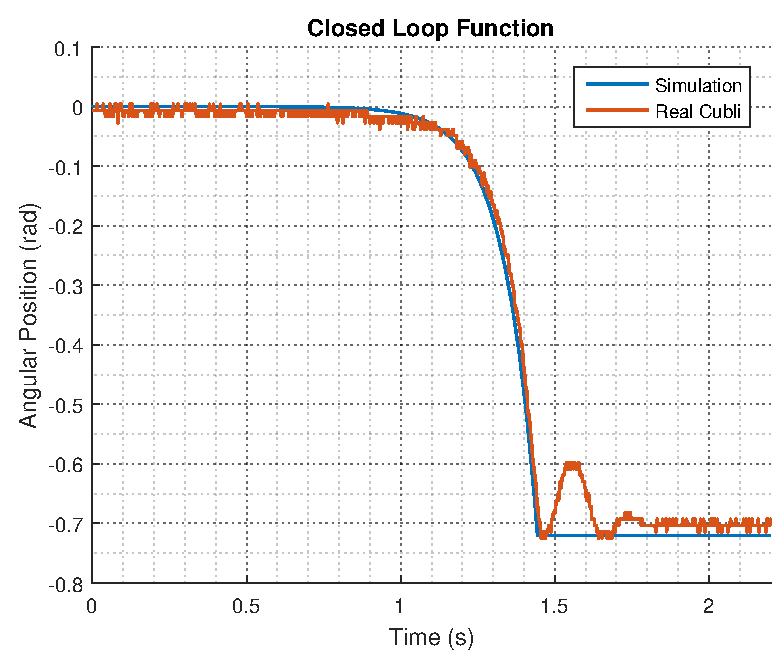
\includegraphics[scale=0.6]{figures/closedLoopResponse}	
	\caption{Behavior of the closed loop function with a proportional controller, both in simulation and reality}
	\label{closedLoopResponse}
\end{figure}
%
It is clear that the closed loop function has an unstable response when a reference of 0 rad is required.
